% Options for packages loaded elsewhere
\PassOptionsToPackage{unicode}{hyperref}
\PassOptionsToPackage{hyphens}{url}
\PassOptionsToPackage{dvipsnames,svgnames,x11names}{xcolor}
%
\documentclass[
]{article}

\usepackage{amsmath,amssymb}
\usepackage{iftex}
\ifPDFTeX
  \usepackage[T1]{fontenc}
  \usepackage[utf8]{inputenc}
  \usepackage{textcomp} % provide euro and other symbols
\else % if luatex or xetex
  \usepackage{unicode-math}
  \defaultfontfeatures{Scale=MatchLowercase}
  \defaultfontfeatures[\rmfamily]{Ligatures=TeX,Scale=1}
\fi
\usepackage{lmodern}
\ifPDFTeX\else  
    % xetex/luatex font selection
\fi
% Use upquote if available, for straight quotes in verbatim environments
\IfFileExists{upquote.sty}{\usepackage{upquote}}{}
\IfFileExists{microtype.sty}{% use microtype if available
  \usepackage[]{microtype}
  \UseMicrotypeSet[protrusion]{basicmath} % disable protrusion for tt fonts
}{}
\makeatletter
\@ifundefined{KOMAClassName}{% if non-KOMA class
  \IfFileExists{parskip.sty}{%
    \usepackage{parskip}
  }{% else
    \setlength{\parindent}{0pt}
    \setlength{\parskip}{6pt plus 2pt minus 1pt}}
}{% if KOMA class
  \KOMAoptions{parskip=half}}
\makeatother
\usepackage{xcolor}
\usepackage[lmargin=1.25in,rmargin=1.25in,tmargin=1in,bmargin=1in]{geometry}
\setlength{\emergencystretch}{3em} % prevent overfull lines
\setcounter{secnumdepth}{5}
% Make \paragraph and \subparagraph free-standing
\makeatletter
\ifx\paragraph\undefined\else
  \let\oldparagraph\paragraph
  \renewcommand{\paragraph}{
    \@ifstar
      \xxxParagraphStar
      \xxxParagraphNoStar
  }
  \newcommand{\xxxParagraphStar}[1]{\oldparagraph*{#1}\mbox{}}
  \newcommand{\xxxParagraphNoStar}[1]{\oldparagraph{#1}\mbox{}}
\fi
\ifx\subparagraph\undefined\else
  \let\oldsubparagraph\subparagraph
  \renewcommand{\subparagraph}{
    \@ifstar
      \xxxSubParagraphStar
      \xxxSubParagraphNoStar
  }
  \newcommand{\xxxSubParagraphStar}[1]{\oldsubparagraph*{#1}\mbox{}}
  \newcommand{\xxxSubParagraphNoStar}[1]{\oldsubparagraph{#1}\mbox{}}
\fi
\makeatother


\providecommand{\tightlist}{%
  \setlength{\itemsep}{0pt}\setlength{\parskip}{0pt}}\usepackage{longtable,booktabs,array}
\usepackage{calc} % for calculating minipage widths
% Correct order of tables after \paragraph or \subparagraph
\usepackage{etoolbox}
\makeatletter
\patchcmd\longtable{\par}{\if@noskipsec\mbox{}\fi\par}{}{}
\makeatother
% Allow footnotes in longtable head/foot
\IfFileExists{footnotehyper.sty}{\usepackage{footnotehyper}}{\usepackage{footnote}}
\makesavenoteenv{longtable}
\usepackage{graphicx}
\makeatletter
\newsavebox\pandoc@box
\newcommand*\pandocbounded[1]{% scales image to fit in text height/width
  \sbox\pandoc@box{#1}%
  \Gscale@div\@tempa{\textheight}{\dimexpr\ht\pandoc@box+\dp\pandoc@box\relax}%
  \Gscale@div\@tempb{\linewidth}{\wd\pandoc@box}%
  \ifdim\@tempb\p@<\@tempa\p@\let\@tempa\@tempb\fi% select the smaller of both
  \ifdim\@tempa\p@<\p@\scalebox{\@tempa}{\usebox\pandoc@box}%
  \else\usebox{\pandoc@box}%
  \fi%
}
% Set default figure placement to htbp
\def\fps@figure{htbp}
\makeatother

\pagenumbering{gobble}
\usepackage{scrlayer-scrpage}
\rohead{Batch Output to Tethys V1.0}
\usepackage[noblocks]{authblk}
\renewcommand*{\Authsep}{, }
\renewcommand*{\Authand}{ and }
\renewcommand*{\Authands}{, }
\renewcommand\Affilfont{\small}
\makeatletter
\@ifpackageloaded{tcolorbox}{}{\usepackage[skins,breakable]{tcolorbox}}
\@ifpackageloaded{fontawesome5}{}{\usepackage{fontawesome5}}
\definecolor{quarto-callout-color}{HTML}{909090}
\definecolor{quarto-callout-note-color}{HTML}{0758E5}
\definecolor{quarto-callout-important-color}{HTML}{CC1914}
\definecolor{quarto-callout-warning-color}{HTML}{EB9113}
\definecolor{quarto-callout-tip-color}{HTML}{00A047}
\definecolor{quarto-callout-caution-color}{HTML}{FC5300}
\definecolor{quarto-callout-color-frame}{HTML}{acacac}
\definecolor{quarto-callout-note-color-frame}{HTML}{4582ec}
\definecolor{quarto-callout-important-color-frame}{HTML}{d9534f}
\definecolor{quarto-callout-warning-color-frame}{HTML}{f0ad4e}
\definecolor{quarto-callout-tip-color-frame}{HTML}{02b875}
\definecolor{quarto-callout-caution-color-frame}{HTML}{fd7e14}
\makeatother
\makeatletter
\@ifpackageloaded{caption}{}{\usepackage{caption}}
\AtBeginDocument{%
\ifdefined\contentsname
  \renewcommand*\contentsname{Table of contents}
\else
  \newcommand\contentsname{Table of contents}
\fi
\ifdefined\listfigurename
  \renewcommand*\listfigurename{List of Figures}
\else
  \newcommand\listfigurename{List of Figures}
\fi
\ifdefined\listtablename
  \renewcommand*\listtablename{List of Tables}
\else
  \newcommand\listtablename{List of Tables}
\fi
\ifdefined\figurename
  \renewcommand*\figurename{Figure}
\else
  \newcommand\figurename{Figure}
\fi
\ifdefined\tablename
  \renewcommand*\tablename{Table}
\else
  \newcommand\tablename{Table}
\fi
}
\@ifpackageloaded{float}{}{\usepackage{float}}
\floatstyle{ruled}
\@ifundefined{c@chapter}{\newfloat{codelisting}{h}{lop}}{\newfloat{codelisting}{h}{lop}[chapter]}
\floatname{codelisting}{Listing}
\newcommand*\listoflistings{\listof{codelisting}{List of Listings}}
\makeatother
\makeatletter
\makeatother
\makeatletter
\@ifpackageloaded{caption}{}{\usepackage{caption}}
\@ifpackageloaded{subcaption}{}{\usepackage{subcaption}}
\makeatother

\usepackage{bookmark}

\IfFileExists{xurl.sty}{\usepackage{xurl}}{} % add URL line breaks if available
\urlstyle{same} % disable monospaced font for URLs
\hypersetup{
  pdftitle={Batch Output to Tethys},
  pdfauthor={Douglas Gillespie},
  colorlinks=true,
  linkcolor={blue},
  filecolor={Maroon},
  citecolor={Blue},
  urlcolor={Blue},
  pdfcreator={LaTeX via pandoc}}


\title{Batch Output to Tethys}


\author[1]{Douglas Gillespie}

\affil[1]{Sea Mammal Research Unit, University of St Andrews}


\date{2025-02-12}
\begin{document}
\maketitle

\centerline{\textbf{Tutorial Version 2.0}}
\vspace{3cm}


\centerline{\textbf{Learning Outcomes}}

In this tutorial you wil learn to output data from multiple PAMGuard datasets
to a Tethys database. The tutorial assumes that you are already familiar
with both Tethys and with the Batch Processing system.

\renewcommand*\contentsname{Table of contents}
{
\hypersetup{linkcolor=}
\setcounter{tocdepth}{3}
\tableofcontents
}

\newpage{}

\pagenumbering{arabic}
\pagestyle{plain}

\section{Prerequisites}\label{prerequisites}

\subsection{Software Versions}\label{software-versions}

To run this tutorial you must have PAMGuard version 2.02.16 or later,
the Batch Processing Plugin, Version 1.8 or later, and Tethys sever
Version 3.2 or later. The Tethys server must be running on your
computer. If you don't have these, or don't know how to set them up,
please complete the batch processing tutorial, and the full PAMGuard
Tethys tutorial available at
\href{https://www.pamguard.org/tutorials/tethys.html}{www.pamguard.org/tutorials/tethys.html}.

\subsection{Sample Data}\label{sample-data}

The data you'll be using for this tutorial are the same data used for
the Batch Processing tutorial. These come from a deployment of five
SoundTrap 300 recorders off the West coast of Scotland, which form part
of the \href{https://www.sams.ac.uk/science/projects/compass/}{Compass
Project}. We've taken a single days data for each recorder since the
full dataset would be too large for a tutorial exercise.

If you completed the batch processing tutorial using different data,
feel free to use those data for this tutorial.

If you completed the Batch Processing Tutorial section on running
offline tasks, you should have a Batch Processing display looking
something like Figure~\ref{fig-offconfig}.

\begin{figure}

\centering{

\pandocbounded{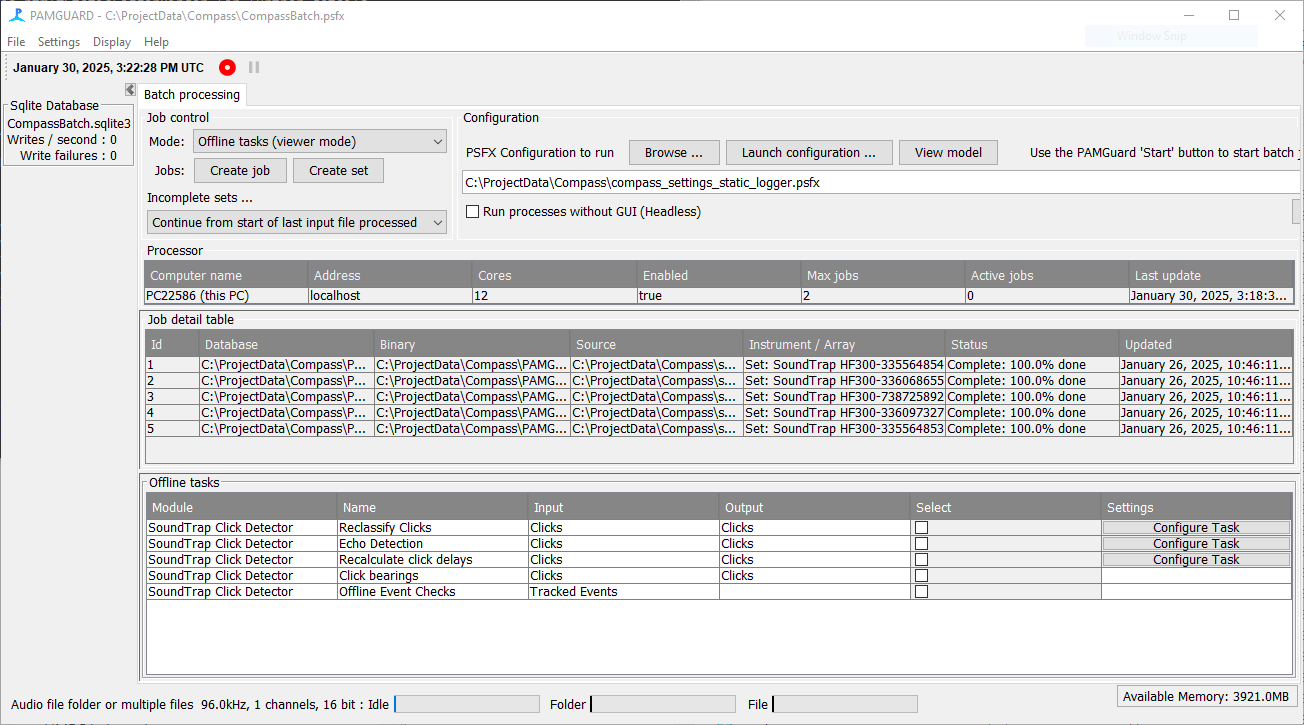
\includegraphics[keepaspectratio]{images/offlineconfig.png}}

}

\caption{\label{fig-offconfig}Configuration display for controlling
offline tasks as it should have looked at the end of the batch
processing tutorial}

\end{figure}%

\section{Setup Tethys}\label{setup-tethys}

Do NOT add a Tethys module to the batch processor configuration. Add it
to the Batch processors \emph{Run Configuration}. To open the \emph{Run
Configuration} click on \emph{Launch Configuration} near the top of the
display, and a new PAMGuard window will open. From the \emph{File/Add
Modules/Utilities} menu, add the Tethys module to the Run Configuration.
Check the Tethys server connection is OK, then close the Run
Configuration.

\begin{tcolorbox}[enhanced jigsaw, arc=.35mm, title=\textcolor{quarto-callout-note-color}{\faInfo}\hspace{0.5em}{Adding a Viewer only module}, opacitybacktitle=0.6, colbacktitle=quarto-callout-note-color!10!white, colframe=quarto-callout-note-color-frame, colback=white, toprule=.15mm, rightrule=.15mm, bottomtitle=1mm, opacityback=0, breakable, toptitle=1mm, coltitle=black, left=2mm, bottomrule=.15mm, leftrule=.75mm, titlerule=0mm]

Note that to add the Tethys module to your Run Configuration, you HAVE
to open the run configuration from within the Batch Processor. This is
because Tethys is normally only available in Viewer mode. Launching from
the batch processor will enable some additional options that allow a
limited subset of Viewer functionality.

\end{tcolorbox}

You don't need to do anything else to your Tethys settings here, and
certainly don't attempt to export any data ! Close the RunConfiguration
and the Batch Processor Oflfine Tasks table will update with 9 addiontal
Tethys export tasks (Figure~\ref{fig-withtethys}).

\begin{figure}

\centering{

\pandocbounded{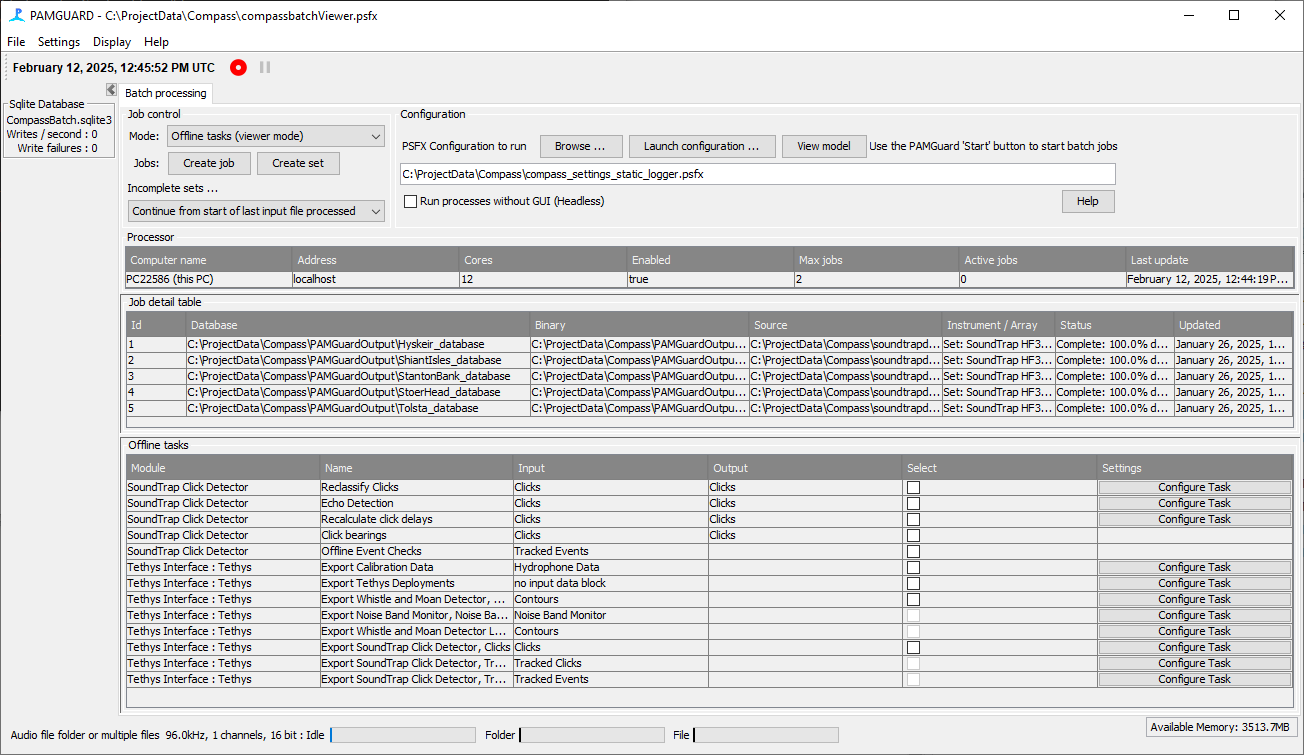
\includegraphics[keepaspectratio]{images/offlineconfigtethys.png}}

}

\caption{\label{fig-withtethys}Configuration display with the additional
Tethys Export tasks when the Tethys module has been successfully added
to the Run Configuration}

\end{figure}%

\subsection{Check your Metadata}\label{check-your-metadata}

When you completed the batch processor tutorial, you should have entered
array / hydrophone specific data for each of the five datasets in the
jobs table. If you didn't do that, you need to do it now, because this
information is essential in managing the relationship between
\href{https://www.pamguard.org/olhelp/utilities/tethys/docs/tethys_mappings.html}{PAMGuard
datasets and Tethys documents}. Above all, make sure that each dataset
has a unique Instrument / Array identifier (Figure~\ref{fig-instid})
unless of course you're exporting multiple datasets from the same
instrument, but collected at different times.

\begin{figure}

\centering{

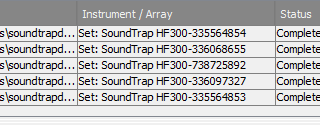
\includegraphics[width=0.45\linewidth,height=\textheight,keepaspectratio]{images/instid.png}

}

\caption{\label{fig-instid}Instrument / Array identification information
in the Batch Jobs table}

\end{figure}%

\subsection{Configure the export
tasks}\label{configure-the-export-tasks}

We want to export the following data for each or our batch datasets:

\begin{itemize}
\tightlist
\item
  Calibration Data
\item
  Tethys Deployments
\item
  Whistle and Moan Detector contours
\item
  Sound Trap Click Detector, clicks
\end{itemize}

Of course, if you're exporting data from a different PAMGuard
configuration, then you'll be seeing a different list of possible export
tasks. Select what you want, but you should always export Calibration
and Deployment data before you export any Detections or Localisations.

You may find that you can't select all of these tasks, because some of
the checkboxes to select those tasks are greyed out. If a task is greyed
out, then hovering the mouse over that task should display a message
saying what's wrong, which usually means that the Tethys Server was not
running, you've not provided required information for that export, or in
the case of Detections have not set up correct
\href{https://www.pamguard.org/olhelp/utilities/tethys/docs/tethys_speciescodes.html}{ITIS
species codes}. For each task, click on the \textbf{Configure Task}
button and enter the required data into the same Wizards that you'd have
seen when you completed the Tethys Tutorial. Hopefully, you entered most
of this information when you were completing the Batch Processing
tutorial with this dataset. If not, refer back to that tutorial and the
\href{https://www.sams.ac.uk/science/projects/compass/}{Compass website}
to find the data you need and enter it now. Once the required
information have been collected you should be able to select the tasks
you want to run.

When setting up the export options for the Whistles and Clicks, I
suggest you export 10 minute bin counts for each type of detection and
require a minimum of at least 10 sounds per bin.

Once you can select the check boxes for all five tasks we want to run,
you're ready to start exporting

\begin{tcolorbox}[enhanced jigsaw, arc=.35mm, title=\textcolor{quarto-callout-note-color}{\faInfo}\hspace{0.5em}{Configuration Differences}, opacitybacktitle=0.6, colbacktitle=quarto-callout-note-color!10!white, colframe=quarto-callout-note-color-frame, colback=white, toprule=.15mm, rightrule=.15mm, bottomtitle=1mm, opacityback=0, breakable, toptitle=1mm, coltitle=black, left=2mm, bottomrule=.15mm, leftrule=.75mm, titlerule=0mm]

Note that a lot the data you enter here is going to be exactly the same
for every dataset that you export. Hopefully, this is a good thing,
since if all the data are from the same project, then the methods,
abstracts, and other information should be the same. However, there may
be a few details, such as dates of calibrations, or there serial numbers
of instruments used to calibrate your hydrophones which are not captured
here.

If you're data genuinely ARE different, then you probably need to export
the data from each set individually, or break it up into smaller sets
for batch processing of data that really are the same.

We always welcome suggests as to how to improve the options in the
PAMGuard user interface.

\end{tcolorbox}

\section{Run the tasks}\label{run-the-tasks}

Assuming that you're using the batch configuration from your earlier
work with the Batch Processing tutorial, all five jobs are probably
marked as complete. Right click on the jobs table and select the menu
item \emph{Reprocess ALL jobs}.

Check the number of jobs you want to run concurrently (2 or 3 is
probably good), then press the red Start button at the top of the
PAMGuard display. As with other offline tasks, the Batch Processor
module will launch PAMGuard configurations for each task, add the Tethys
module, then run the tasks before slosing those configurations.

Running these export tasks on the given data should take about five
minutes.

\begin{figure}

\centering{

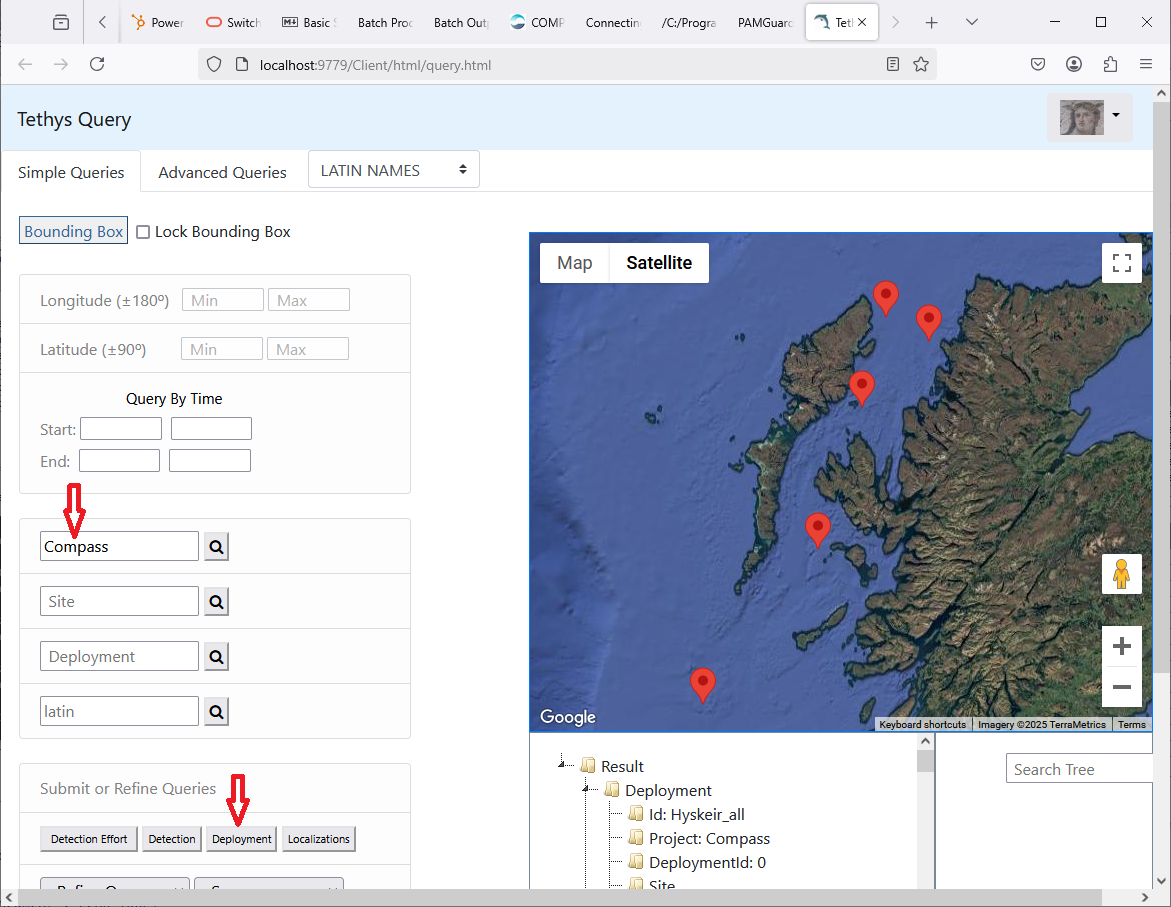
\includegraphics[width=0.95\linewidth,height=\textheight,keepaspectratio]{images/client.png}

}

\caption{\label{fig-client}Tethys Client showing the locations of the
datasets exported during this tutorial}

\end{figure}%

\section{Look at the data}\label{look-at-the-data}

Open the Tethys client Program (usually
\url{http://localhost:9779/Client/html/query.html}). Enter the Project
Name as Compass and press the Deployment button near the bottom of the
screen (Figure~\ref{fig-client}). Zoom in on the map to the West coast
of Scotland and you should see five markers indicating the positions of
the SoundTrap deployments.

Refer to the Tethys Documentation for other ways to look at the exported
data using the Client, Data Explorer, R, and Matlab.




\end{document}
